\documentclass[11pt, fullpage,letterpaper]{article}

\usepackage[margin=1in]{geometry}
\usepackage{url}
\usepackage{amsmath}
\usepackage{amssymb}
\usepackage{xspace}
\usepackage{graphicx}
\usepackage{hyperref}
\usepackage{listings}

\newcommand{\semester}{Spring 2019}
\newcommand{\releaseDate}{27 Apr, 2019}
\newcommand{\dueDate}{11:59pm, 24 Apr, 2019}

\newcommand{\bx}{{\bf x}}
\newcommand{\bw}{{\bf w}}

\title{Pharming Detection \semester}
\author{Lee S. Leavitt}

\begin{document}
\maketitle
\newcommand{\Hcal}{\mathcal{H}} 

\section{Introduction}
This project can be found at the github respository \href {}{}Constellation Pharmacology is an assay that looks at a dissociated tissue of interest. In this case the dorsal root ganglion (DRG), the an organ of the body responsible for all physical sensations (heat, cold, pain, proprioception, light touch, heavy touch). The tissue is;
\begin{enumerate}	
\item Gently broken up until the cells in this tissue (neurons) are isolated from one another. 
\item The cells, $\approx 5000$, are plated so that each cell is seperate from one another.
\item The are loaded with a dye \href{https://www.ncbi.nlm.nih.gov/pmc/articles/PMC2763293/}{fura2}, a dye which allows for the measure of calcium into and out of the cell.
\item Varieties of natural products are applied to the cell, which produce unique response in subsets of the neurons while a video is collected. The natural products applied are;
	\begin{enumerate}
		\item Allyl isothiocynate (\href{https://en.wikipedia.org/wiki/Allyl_isothiocyanate}{AITC}) the main compenent in mustard oil, and wasabi.
		\item \href{https://en.wikipedia.org/wiki/Menthol}{Menthol}, the compound found in peppermint which evokes a cooling sensations. 
		\item \href{https://en.wikipedia.org/wiki/Capsaicin}{Capsaicin}, the spicy component of chili peppers. 
		\item Potassium ($K^+$) at a concetration of 40mM, which activates a variety of voltage gated ion channels on the surface of these cells.
		\begin{center}
		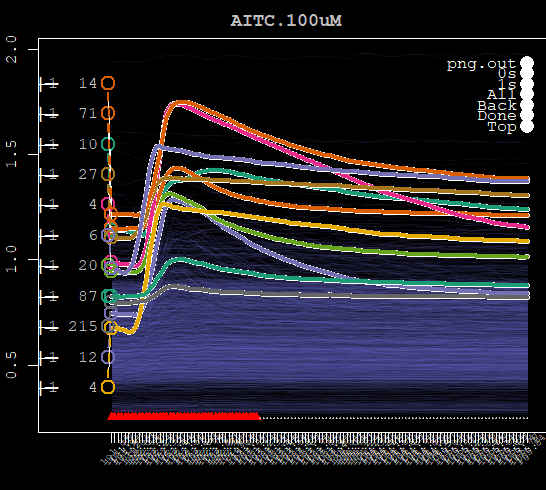
\includegraphics[scale=.3]{AITC_img.png}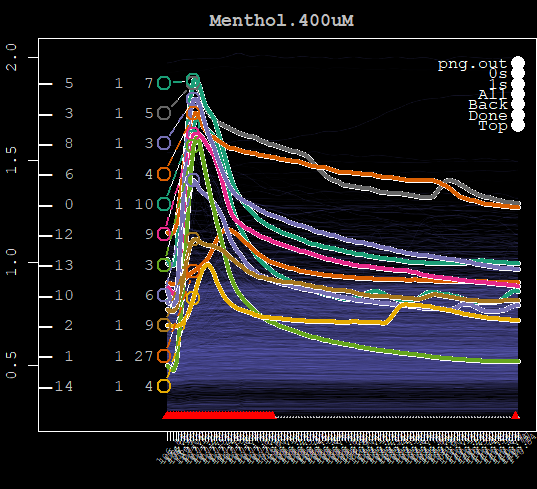
\includegraphics[scale=.3]{MENTH_img.png}
		\newline
		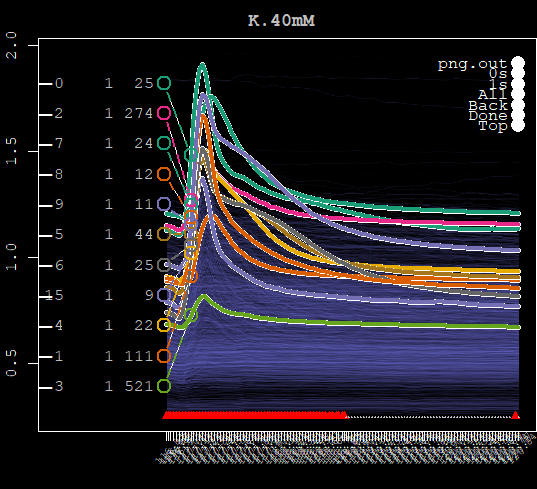
\includegraphics[scale=.3]{K40_img.png}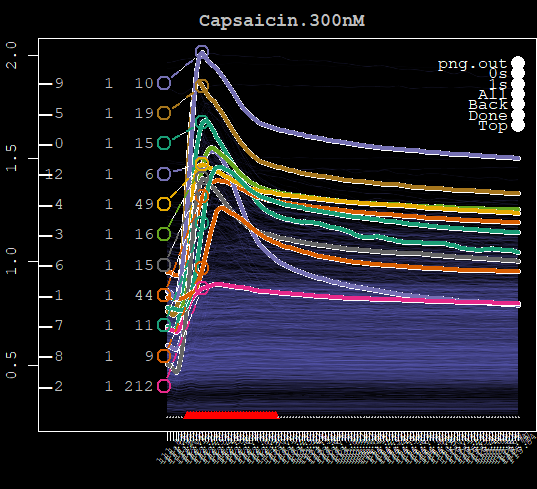
\includegraphics[scale=.3]{CAPS_img.png}
		\end{center}


	\end{enumerate}
\end{enumerate}
Then using an open source software, CellProfiler, cells are identified based on whether they are loaded with the fura2 dye. Each cell is considered a region of interest (ROI). Within each frame, each ROIs mean intensity is collected. Each intenisty is compiled into a $n$, by $d$ matrix where $n = time$, and $d = cell$. The traces then undergo a significat cleaning step;
\begin{enumerate}
	\item Padding: 3 points are added to the end of each trace since the last natural product application does not allow the trace baseline to return  to the bottom (for example Capsaicin), three points are added allowing a better representation of the trace.
	\item Despiking and smoothing: The traces vary in the ammount of general noise.  In addition to this, since this assays uses fluorescent imaging many dust particles are very fluorescent.  To obtian an accurate reading of peak height these aberant values are taken out. 
	\item Baseline Correction: The baseline is then corrected. This means the trace is corrected to correct for upward baseline drift, moves everything to a zero base.
	\item Normalization: K 40mM and Capsaicin induce a maximal response. This maximal response is then considered 1, where the minimum value is now considered 0.

\end{enumerate}
The scientists then use a in house application to correct an automatic binary scoring. The images above cooresponding to each natural product application shows the diversity of responses. This process is aided by hierarchal clustering. This techniques allows to scientist to view and obttain a view of all cells, while correcting the scoring.

Statistics are generated for each natural product application. The statistics below show the statistics generated for the feature space.

\begin{enumerate}
\item snr: Signal to Noise Ratio provide a measure of peak sharpness.  This statistic has proven to be most useful for menthol, and least significant for Capsaicin since the Capsaicin response does not return to baseline.
\item tot: Sum of all point within a window region of 4 minutes. General measure of area.
\item max: maximun value within the region of application.
\item ph.a.r: Peak height to area ratio.
\item wm: where does the maximun value occur.
\end{enumerate}

\section{Data Processing}
This was the most time consuming and difficult aspect of the project. Since we have not dedicated time to generating a database, each experiment is stored in an R list of dataframes, and lists.  In addition to this each scientist spells each natural product differently, applies each natural product different orders. Significant time went into building an flexible application to allow for growing a significant feature and label space. After a significant ammount of data wrangling 58,301 instances were collected.

\section{Support Vector Machine}

The goal of this experiment was to determine whether a response could be detected at a significant rate. Initially the e1071 package was used to produce the SVM. This package produced fantastic results. After this, radial svm was attempted to see if this could further improve the model. Suprsingly radial SVM takes significantly longer than linear. Where the majority of the time comes from is for the tuning of the $C$ and $\sigma$ value. Due to this extensive ammount of time required to tune the radial SVM, the $caret$ package was invoked and used for tuning.  What is most nice about the caret package is the ability to paralleize the code. with e1071 my processors utilization was $\approx 20\%$. After parallelization my processors were at 100\% and was able to cross validate.

\begin{enumerate}
	\item Linear vs Radial SVM: The first experimentor included a single experimentors data which is 30,000 instances. For linear SVM it was cross Validated (10 fold, repeated 4 times), and 12 C values were tested for each natural product. The training data was selected as a random sample of \frac{2}{3} of the total dataset. Train vs test accuracy matched very closely for each experiment.
		\begin{center}
		\begin{tabular} {c|cccc}
			SVM Method & AITC & Menthol & Capsaicin & K.40mM \\ \hline \hline
			linear & 92\% & 92.94\% & 97.8\% & 97.9\% \\ \hline
			radial & 93\% & 93.6\% & 98\% & 98.5\% \\ \hline
		\end{tabular}
	\end{center}	
	\item The W vector produced from the linear SVM also provides significant insight into what feature has the greatest effect on the fit. As can be observed below the most important feature for defining the hyperplane is the signal to noise ratio (snr), whereas a majority of the other features do not help in defining the hyperplane.
	\begin{center}
		\begin{tabular}{c|ccccc}
			''& snr & tot & max & ph.a.r & wm \\ \hline \hline
			AITC & 4.49 & 0.42 & -0.42 & -0.33 & -0.17 \\ \hline
			Menthol & 2.93 & 0.04 & 0.06 & -0.52 & -0.26 \\ \hline
			Capsaicin & 5.41 & -0.07 & 0.39 & -0.06 & -0.56 \\ \hline
			K.40mM & 5.13 & -0.55 & 0.77 & -0.00 & -0.81 \\ \hline
		\end{tabular}
	\end{center}
\end{enumerate}


\section{Future Directions}
\begin{enumerate}
\item It would be nice to move our data into a database format. This would allows for a much faster data collection and testing method. Currently each experiment is $\approx 500-1,500 MB$ Only a subset of this information needs to be accessed as well, thus a significant ammount of time was spend troublshooting the loading features and label space into the support vector machine.  

\item Auditing: The next series of our application that needs to be developed is a way to view the support vectors. These cells should have a some significant value for helping us tune the statistics collected, along with improving the data cleaning protocol. I have already developed a UI within the R environment while works in rapid way for displaying the data.

\item Our data scientist has developed a way of obtianing more advanced statsitics by fitting polynomials to the trace shapes. This would be the next set of experiments i would like to run, although this will take a very long time to complete, not to mention the painstakinly difficult process of organizing our messy data.

\item Now that SVM's have proven to been very useful for us during these simple experiment, more advanced effect detection would be interesting to observe and continue development on. In the figure below is an example of the more advanced effects our group would like to detect. a compound pl14a.10uM is applied, and this application causes the cells to have an amplified response to this compound. THis effect is repeated three times.  Unfortuneatly this example is the cleanest as others have significantly more suddle effects.
\newline 
\begin{center}
	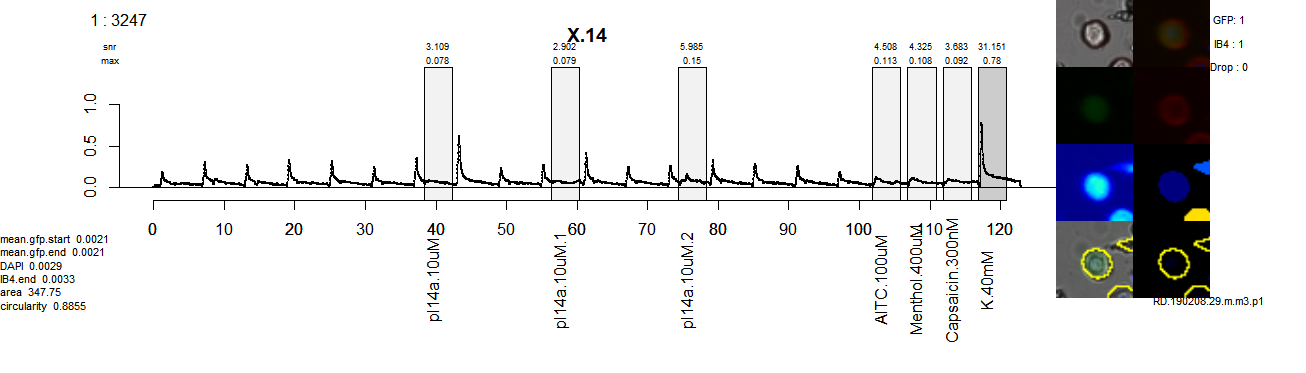
\includegraphics[scale=.3]{advanced_detection.png}
\end{center}
\end{enumerate}

\end{document}